\chapter{METHODOLOGY}\label{chap:METHODOLOGY}
\hspace{0.5in}This chapter describes the techniques we have selected for designing and implementing the Face Replacement System in more detail, and also the techniques we have discovered on our own. This chapter contains the system functions including explanation diagrams.

\section{Face Replacement System Functions}
The Face Replacement System can be described as these following five main functions.

\subsection{Face Detection using OpenCV}

\hspace{0.5in}The first function of the system is face detection. Firstly, the region of each face is detected by the face detector. The face detector detects the existence and the location of the faces in each image. Then, we continue to detect eyes and mouth from this face to get their positions.

\begin{figure}[htb]
   \centering
   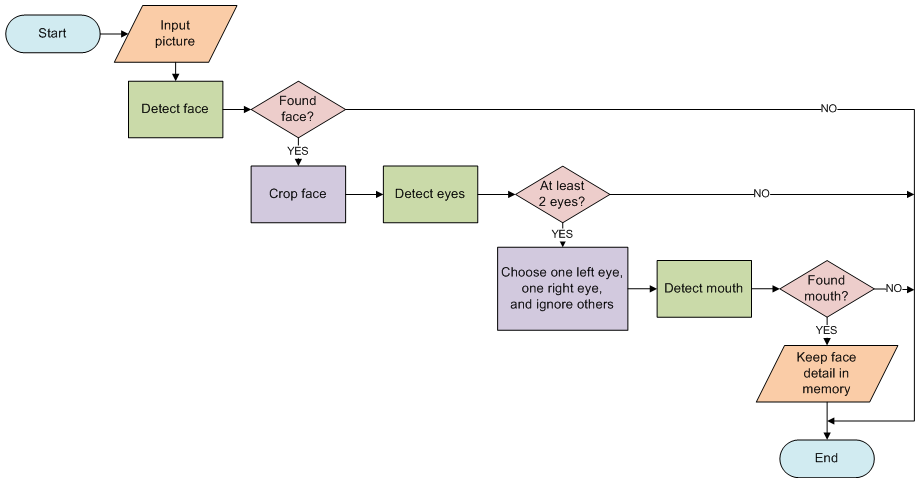
\includegraphics[width=14cm]{F1_FaceDetection.png}
   \caption{Face Detection Flow Chart}
   \label{fig:FaceDetectionDiagram}
\end{figure}

\begin{figure}[htb]
   \centering
   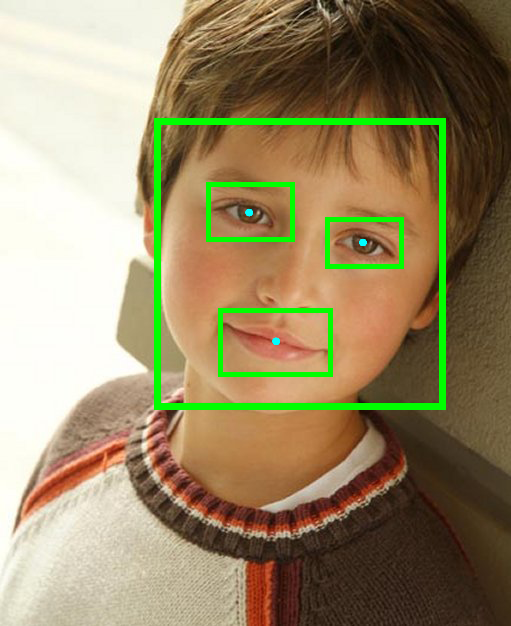
\includegraphics[width=5cm]{facedetection.png}
   \caption{Face Detection}
   \label{fig:FaceDetection}
\end{figure}

\subsection{Face Contour Creation}

\hspace{0.5in}The second function of the system is face contour creation. Our approach is to infer the face contour from main face features that can be obtained easily; two eyes and a mouth. We assume that these features are placed at a similar position for all people, so we may use these features to infer other face features that the face detector cannot detect; for this case, the face contour.

\begin{figure}[htb]
   \centering
   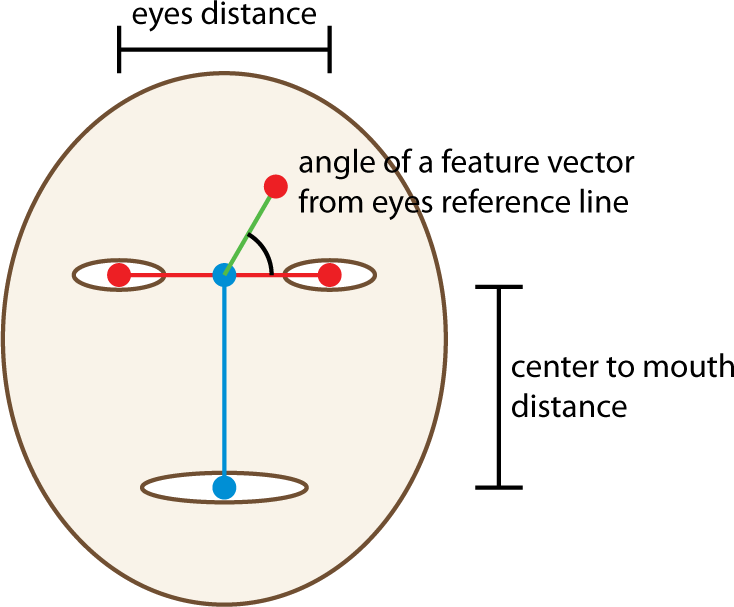
\includegraphics[width=4.5cm]{contourAngle.png}
   \caption{Angle from the Reference Line}
   \label{fig:AngleFromTheReferenceLine}
\end{figure}
\begin{figure}[htb]
   \centering
   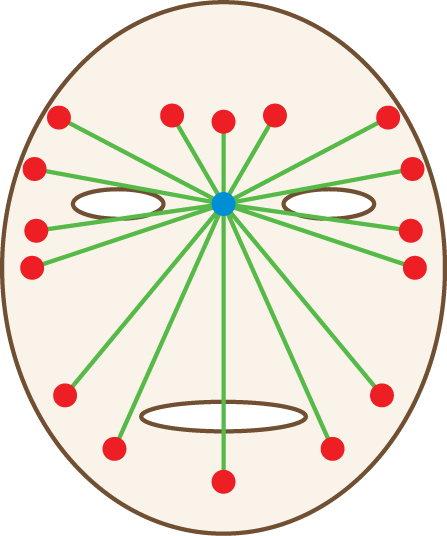
\includegraphics[width=3cm]{contourVectors.png}
   \caption{Face Contour Vectors from the Center Point}
   \label{fig:FaceContourVectorsFromTheCenterPoint}
\end{figure}

Creating a contour begins with getting the eyes and mouth position from the face detector, then calculating the center position between two eyes, and then creating the vector from the center position by using the predefined relationship between the eyes-mouth and face contour to get 16 contour positions around the face area and formed to be a face contour. Each predefined relationship defines the length of the vector from the center and the angle value from the reference line (the line between eyes) to the contour vector.

The raw data of absolute positions of each face has no meaning. The average of absolute positions cannot be used to infer any relationship because faces are placed at different positions, have different pose angles, and have different resolutions. The predefined relationship is gathered by calculating the relative position which is independent from those differences.

To improve the correctness of the predefined relationship, we find the average of each face contour position. As the human face is bi-symmetric, we also find the average between the left and right part of each face.

\begin{figure}[htb]
   \centering
   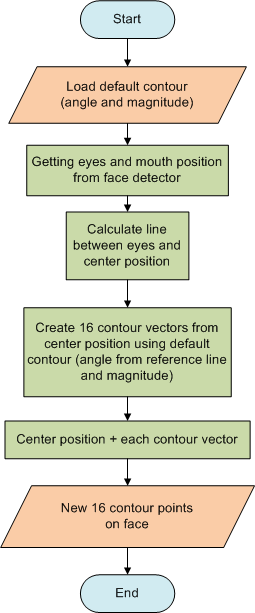
\includegraphics[width=4cm]{F2_FaceContourCreation.png}
   \caption{Face Contour Creation Flow Chart}
   \label{fig:FaceContourCreationFlowchart}
\end{figure}

\begin{figure}[htb]
   \centering
   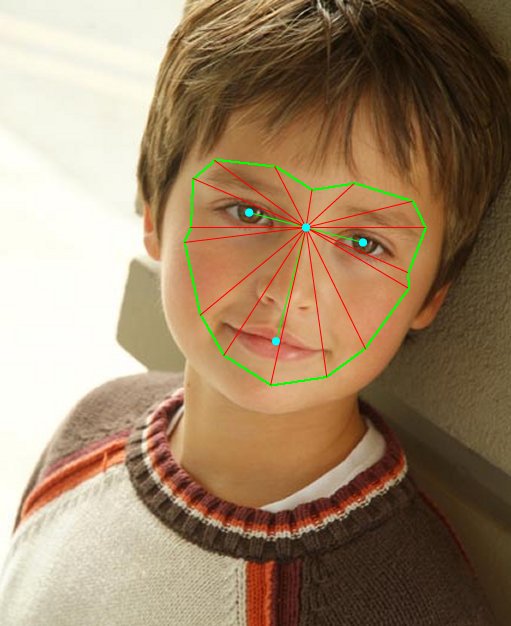
\includegraphics[width=5cm]{facecontourcreation.png}
   \caption{Contour Creation}
   \label{fig:ContourCreation}
\end{figure}

\subsection{Alignment}

\hspace{0.5in}The third function of the Face Replacement System is alignment. Alignment is another important factor in order to create a more realistic result.

\begin{figure}[htb]
   \centering
   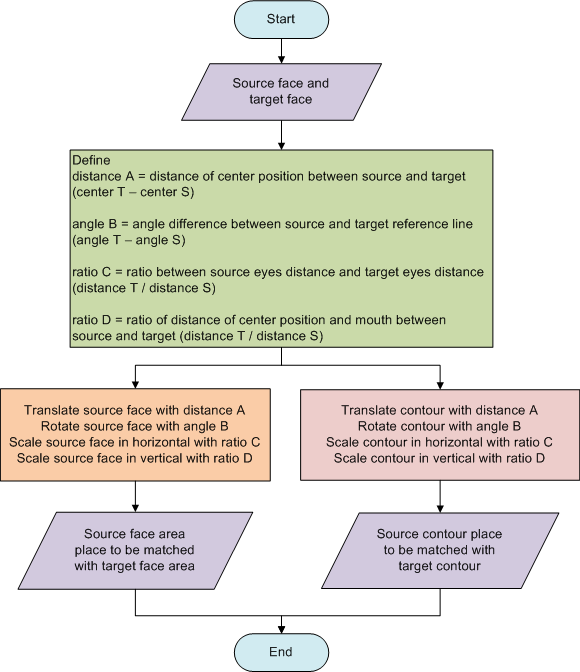
\includegraphics[width=10cm]{F3_Alignment.png}
   \caption{Alignment Flow Chart}
   \label{fig:AlignmentFlowchart}
\end{figure}

The purpose of alignment is to have the eyes and mouth position of the source face to be at the same position as the target face. First, we get the eyes and mouth position of each face from the face detector. To do alignment, we translate the center position of the source face to match the center position of the target face. For rotation, we have to calculate the pose angle difference, and then compensate the pose angle of the source face to match the pose angle of the target face. For scaling, there are two parts. The first part is scaling on the horizontal direction in proportion to the distance between two eyes. The other part is scaling on the vertical direction in proportion to the distance between the center position and mouth. When those three transformations are applied, the alignment will match the source face to the target face.

\begin{figure}[htb]
   \centering
   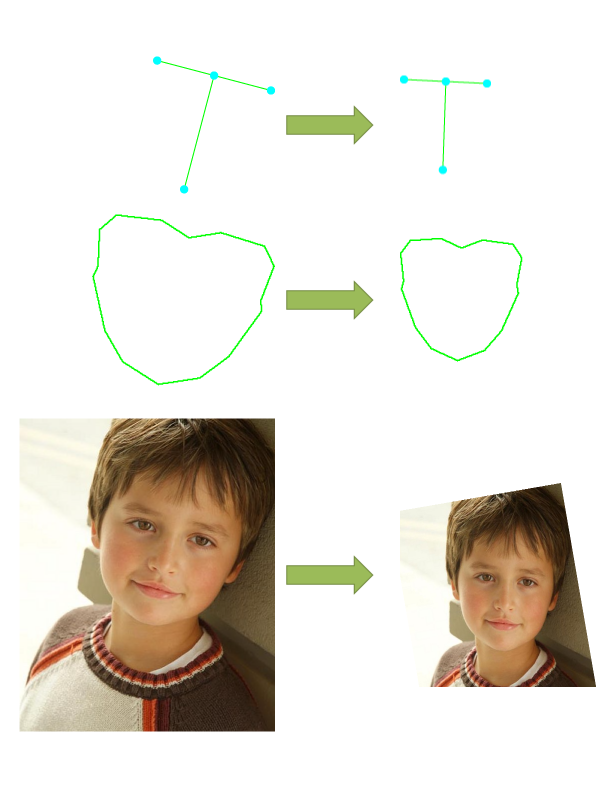
\includegraphics[width=8cm]{alignment.png}
   \caption{Alignment}
   \label{fig:Alignment}
\end{figure}

\subsection{Color Adjustment}

\hspace{0.5in}The fourth function of the system is color adjustment. While the blending process tries to adjust the color of all pixels on the face patch to compensate color differences between source and target pixels along the contour, the face patch will be adjusted regardless of color space limitation. Because a color space has a finite boundary, it is possible for the face patch to be saturated, e.g. too bright. The color transfer technique is optionally used to reduce those effects by mapping the color range statistically before passing to the blending process. Then the blending process will receive the face patch in which the colors are already almost the same, and then make changes only to minor differences on the boundary area.

Because the lighting problems are still found in the results, we have modified the color transfer to map colors by their percentiles. This approach can transfer some characteristics, i.e. the proportion of dark pixels and bright pixels will be preserved. The distribution of color is not just relocated to the same range but also be cloned as the same shape as shown in figure~\ref{fig:ColorTransfer}.

\begin{figure}[htb]
   \centering
   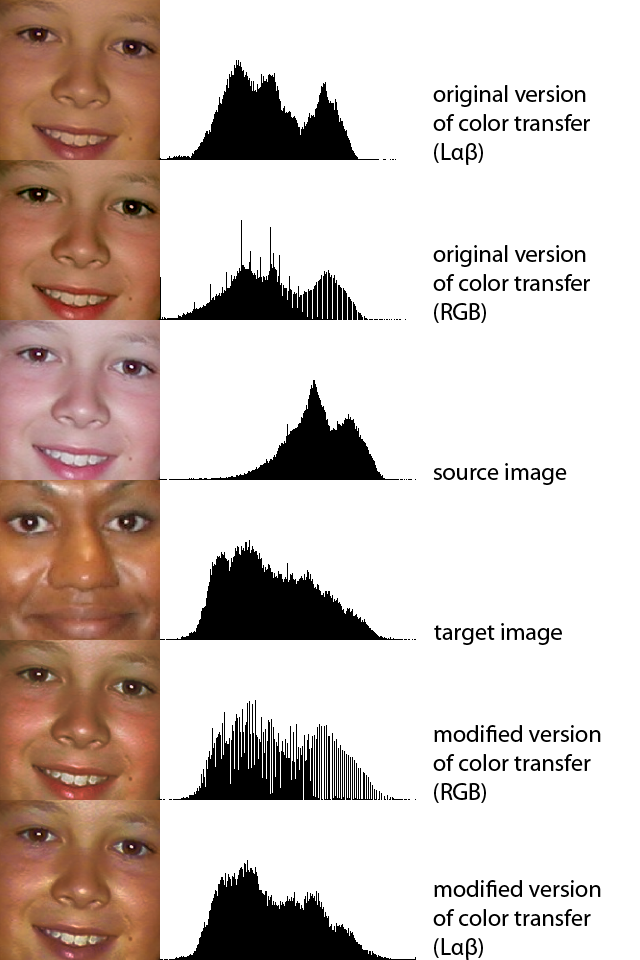
\includegraphics[width=8.5cm]{colorTransfer.png}
   \caption{Color Transfer Techniques Comparison with Histogram}
   \label{fig:ColorTransfer}
\end{figure}

\begin{figure}[htb]
  \centering
  \subfloat[][Before]{\label{fig:BeforeColorTransfer}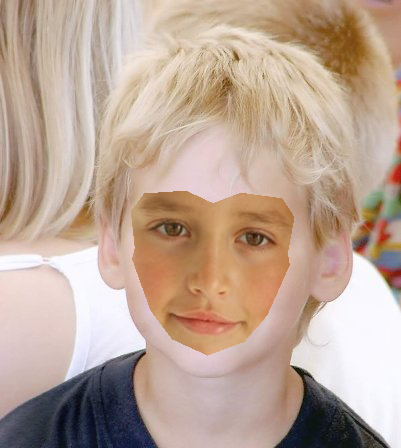
\includegraphics[width=0.3\textwidth]{beforeColorTransfer.png}}
  \subfloat[][After]{\label{fig:AfterColorTransfer}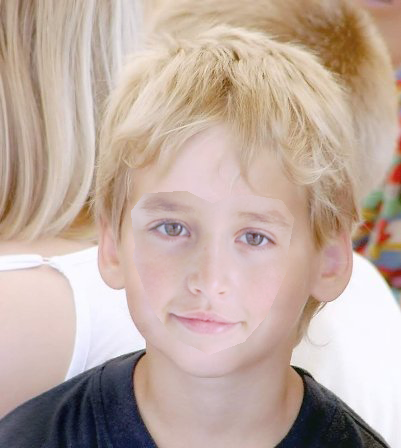
\includegraphics[width=0.3\textwidth]{blendingbefore.png}}
  \caption{Color Adjustment Result}
  \label{fig:ColorAdjustmentResult}
\end{figure}

\subsection{Blending}

\hspace{0.5in}The last function of the system is blending. This part attempts to blend two pictures that may have different colors. We try to cancel the color discontinuity between inner and outer pixels along the compositing boundary. The pixels inside the boundary have to be adjusted to match the pixels outside the boundary.

\begin{figure}[htb]
  \centering
  \subfloat[][Before]{\label{fig:BlendingBefore}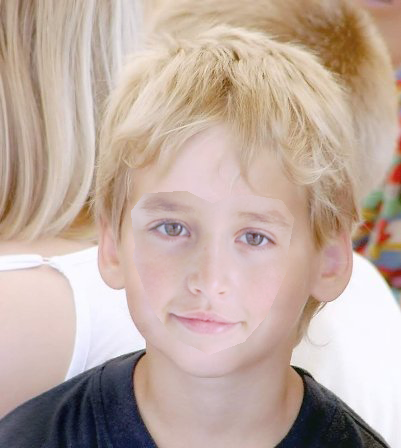
\includegraphics[width=0.3\textwidth]{blendingbefore.png}}
  \subfloat[][After]{\label{fig:BlendingAfter}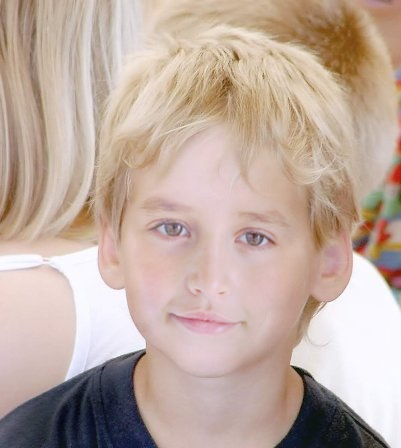
\includegraphics[width=0.3\textwidth]{blendingafter.png}}
  \caption{Blending Result}
  \label{fig:BlendingResult}
\end{figure}

There are 3 inputs for this process, which are source face image as foreground, target face image as background, and mask as a boundary information. The approach begins with rendering the mask of the source image from the contour, and then aligning the source face and the mask to be the same alignment as the target face. The next step is to blend the color of the source and target image along the boundary of the masking area, and the result will be as shown in the figure~\ref{fig:PoissonIdea}.

\begin{figure}[htb]
   \centering
   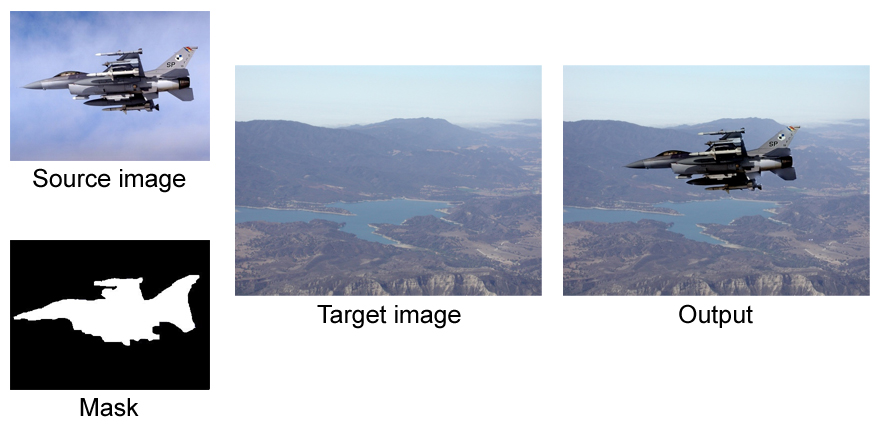
\includegraphics[width=10cm]{poisson-idea.jpg}
   \caption{Poisson Seamless Cloning Example}
   \label{fig:PoissonIdea}
\end{figure}

The techniques we have selected to do this process are Poisson Cloning and Mean-Value Coordinates Cloning.

\subsubsection{Poisson Cloning}
\hspace{0.5in}Poisson Cloning is one of the methods developed by P\'{e}rez et al\cite{Perez2003} for doing seamless cloning between images.

The process begins with calculating the gradient field by calculating the second derivative of color value of those N pixels inside the boundary using the Laplacian operator.

\begin{figure}[htb]
   \centering
   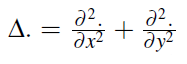
\includegraphics[width=3cm]{laplacian_op.png}
   \caption{Laplacian Operator}
   \label{fig:LaplacianOperator}
\end{figure}

The process subtracts the nearby values both in the X axis and Y axis of the foreground in order to get the first derivatives, then the process does the same with the first derivatives to get the second derivatives of both axes, then it adds both second derivatives together to get the gradient field as shown in figure~\ref{fig:LaplacianMatrix}

\begin{figure}[htb]
   \centering
   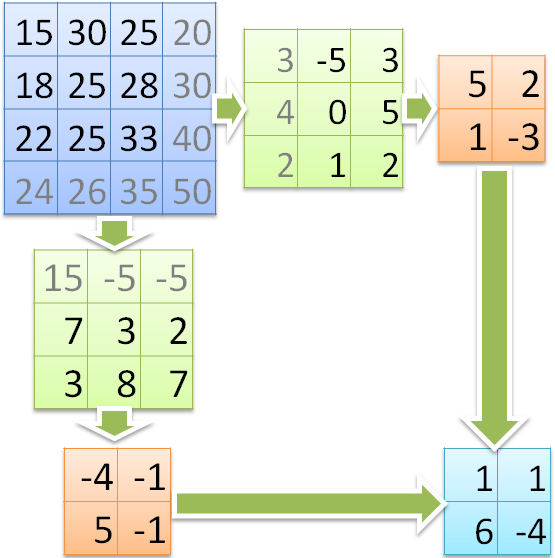
\includegraphics[width=7cm]{laplacian_matrix.png}
   \caption{Laplacian Operation with the Matrix of Pixel Values in the Image}
   \label{fig:LaplacianMatrix}
\end{figure}

Then, we map these gradient values of those N pixels into the vector b. The pixels at the boundary of the contour will be subtracted by the color value of its neighbor pixels of the target face image in order to set the constraint that the pixels inside the boundary must match with pixels outside the boundary.

Next, we express the influence relationship of each inside pixel to its neighbor pixels into the matrix A. Each pixel inside the boundary area will correspond with a column or a row of the matrix. The total N pixels will result in the matrix A sized N${\times}$N. Each column of the matrix will consist of a relationship between the pixels itself and its neighbor pixels. We have to solve the linear equation Ax = b to get the vector x which yields N color values of the final result, then we map those N values back to inside pixels.

\begin{figure}[htb]
   \centering
   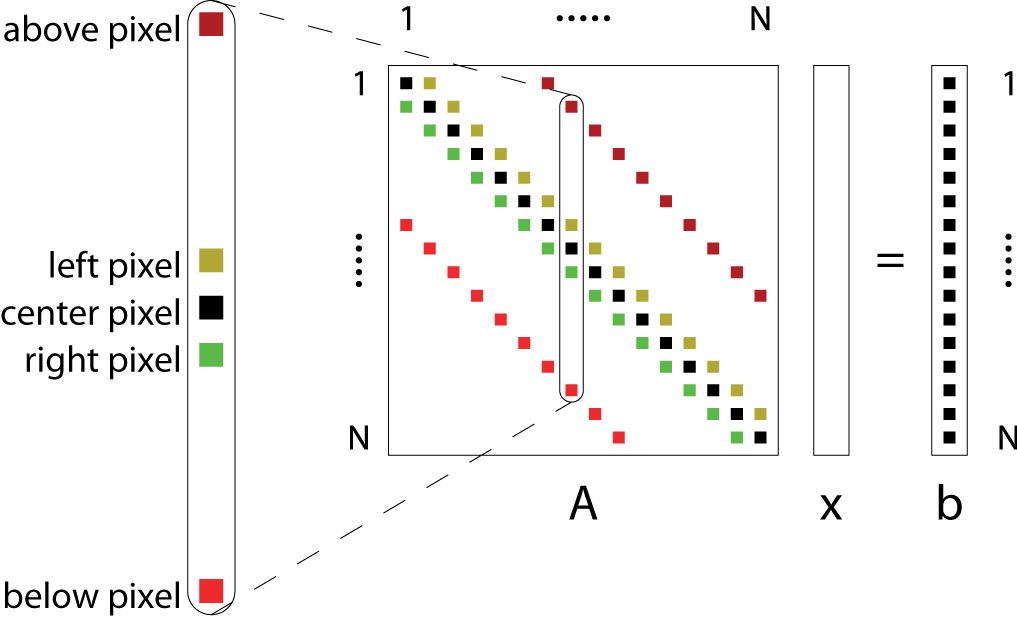
\includegraphics[width=8cm]{poissonMatrix.png}
   \caption{Solving Poisson Equation}
   \label{fig:SolvingPoissonEquation}
\end{figure}

\subsubsection{Mean-Value Coordinates Cloning}
\hspace{0.5in}Mean-Value Coordinates Cloning is another method developed by Farbman et al\cite{Farbman2009} to do seamless cloning between images. This method needs the same inputs as Poisson Cloning. The idea of this method is to create an error correction to cancel color discontinuity around the border. Rather than solving a large linear system, this method finds the interpolation of correction at each interior pixel which is corresponding to Mean-Value Coordinates. Mean-Value Coordinates will determine different mixtures of values along the boundary according to the coordinate by defining a weighted combination of each pixel. Angle and distance, which are calculated from coordinates, are parameters that are used to determine the weighted combination. The weighted combination value of each pixel tells how much the portion of each color difference around the contour will affect to the interior pixel.

\begin{figure}[htb]
   \centering
   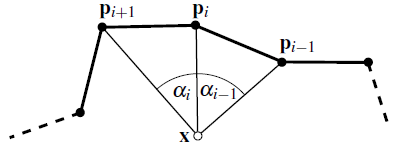
\includegraphics[width=6cm]{mvc.png}
   \caption{Mean-Value Coordinates Cloning}
   \label{fig:MVC}
\end{figure}

From the figure~\ref{fig:MVC}, Pixel x will be affected by the all pixels p on the contour with weights. Each pixel p has corresponding color differences between source and target pixels. The larger angle between pixel p, pixel x, and the next contiguous pixel p means the dominant of the p in that area, so we assign more weight to affect the pixel x. Also the shorter distance between pixel x and each pixel p, the more the weight will be affected by the color differences. If pixel x is located at the center of the inside area, it is likely to have equal weights for all pixels p, so it will be adjusted by a neutral mixture of all pixels p. The pixel x near the contour is likely to be biased to the nearest pixel p, so it will be mostly adjusted by the color difference of that pixel p to make the border looks seamless by achieving almost the same color. 